%% LyX 1.6.4 created this file.  For more info, see http://www.lyx.org/.
%% Do not edit unless you really know what you are doing.
\documentclass[twocolumn,english,prl]{revtex4}
\usepackage[T1]{fontenc}
\usepackage[utf8]{inputenc}
\usepackage{color}
\usepackage{float}
\usepackage{amsmath}
\usepackage{graphicx}
\usepackage{amssymb}

\makeatletter
%%%%%%%%%%%%%%%%%%%%%%%%%%%%%% Textclass specific LaTeX commands.
\@ifundefined{textcolor}{}
{%
 \definecolor{BLACK}{gray}{0}
 \definecolor{WHITE}{gray}{1}
 \definecolor{RED}{rgb}{1,0,0}
 \definecolor{GREEN}{rgb}{0,1,0}
 \definecolor{BLUE}{rgb}{0,0,1}
 \definecolor{CYAN}{cmyk}{1,0,0,0}
 \definecolor{MAGENTA}{cmyk}{0,1,0,0}
 \definecolor{YELLOW}{cmyk}{0,0,1,0}
 }

%%%%%%%%%%%%%%%%%%%%%%%%%%%%%% User specified LaTeX commands.
\newcommand{\pq}[2]{#1\,{\rm #2}}% physical quantity, value and unit
\renewcommand{\Re}{{\rm Re}\,}% real part
\newcommand{\Ej}{E_{\rm J}}% Josephson energy
\newcommand{\Tn}{T_{\rm N}}% Noise temperature
\newcommand{\Rn}{R_{\rm N}}% Normal state resistance
\newcommand{\pairrate}{\Gamma^{\rm cp}}\newcommand{\photonrate}{\Gamma^{\rm ph}}\newcommand{\znorm}{r}

\makeatother

\usepackage{babel}

\begin{document}

\title{Demonstrating quantum speed-up in a superconducting two-qubit processor }


\author{A. Dewes$^{1}$, R. Lauro$^{1},$ F.R. Ong$^{1},$ V. Schmitt$^{1}$,
P. Milman$^{2,3}$, P. Bertet$^{1}$, D. Vion$^{1}$, and D. Esteve$^{1}$}


\affiliation{$^{1}$Service de Physique de l'Etat Condens{é}/IRAMIS/DSM (CNRS
URA 2464), CEA Saclay, 91191 Gif-sur-Yvette, France}


\affiliation{$^{2}$Laboratoire Matériaux et Phénomènes Quantiques, Université
Paris Diderot, 10 rue Alice Domon et Léonie Duquet, 75205 Paris, France, }


\affiliation{$^{3}$Univ. Paris-Sud 11, Institut de Sciences Moléculaires d'Orsay
(CNRS), 91405 Orsay, France}


\date{\today}
\begin{abstract}
We operate a superconducting quantum processor consisting of two tunable
transmon qubits coupled by a swapping interaction, and equipped with
non destructive single-shot readout of the two qubits. With this processor,
we run the Grover search algorithm among four objects and find that
the correct answer is retrieved after a single run with a success
probability between $0.52$ and $0.67$, significantly larger than
the $0.25$ achieved with a classical algorithm. This constitutes
a proof-of-concept for the quantum speed-up of electrical quantum
processors. 
\end{abstract}
\maketitle
The proposition of quantum algorithms \cite{search,Shor,NielsenChuang}
that perform useful computational tasks more efficiently than classical
algorithms has motivated the realization of physical systems \cite{QC}
able to implement them and to demonstrate quantum speed-up. The versatility
and the potential scalability of electrical circuits make them very
appealing for implementing a quantum processor built as sketched in~Fig.
\ref{fig:blueprint}. Ideally, a quantum processor consists of a scalable
set of quantum bits that\textcolor{black}{{} can be efficiently reset,
that can follow any unitary evolution needed by an algorithm using
a universal set of single and two qubit gates, and that can be read
projectively} \cite{divincenzo}. The non-unitary projective readout
operations can be performed at various stages of an algorithm, and
in any case at the end in order to get the final outcome. Quantum
processors based on superconducting qubits have already been operated,
but they fail to meet the above criteria in different aspects. With
the transmon qubit \cite{Transmon Koch,TransmonSchreier} derived
from the Cooper pair box \cite{box}, two simple quantum algorithms,
namely the Deutsch-Jozsa algorithm \cite{DeutschJozsa} and the Grover
search algorithm \cite{search}, were demonstrated in a two qubit
processor with the coupling between the qubits mediated by a cavity
also used for readout \cite{dicarlo}. In this circuit, the qubits
are not read independently, but the value of a single collective variable
is determined from the cavity transmission measured over a large number
of repeated sequences. By applying suitable qubit rotations prior
to this measurement, the density matrix of the two-qubit register
was inferred at different steps of the algorithm, and found in good
agreement with the predicted one. Demonstrating quantum speed-up is
however more demanding than measuring a collective qubit variable
since it requests to obtain an outcome after a single run, i.e. to
perform the single-shot readout of the qubit register. Up to now,
single-shot readout in superconducting processors has been achieved
only for phase qubits \cite{yamamoto,mariantoni}. In a two phase-qubit
processor equipped with single-shot but destructive readout of the
qubits, the Deutsch-Jozsa algorithm \cite{DeutschJozsa} was demonstrated
in \cite{yamamoto} with a success probability of order $0.7$ in
a single run, to be compared to $0.5$ for a classical algorithm. 

Since the Deutsch-Jozsa classification algorithm is not directly related
to any practical situation, demonstrating quantum speed-up for more
useful algorithms in an electrical processor designed along the blueprint
of Fig.~\ref{fig:blueprint} is an important goal. In this work,
we operate a new two transmon-qubit processor \cite{processor} that
comes closer to the ideal scheme than those previously mentioned,
and we run the Grover search algorithm among four objects. Since,
in this case, the algorithm ideally yields the answer after one algorithm
step, its success probability after a single run provides a simple
benchmark. We find that our processor yields the correct answer at
each run with a success probability that ranges between $0.52$ and
$0.67$, whereas a single step classical algorithm using a random
query would yield the correct answer with probability $0.25$. 

%
\begin{figure}
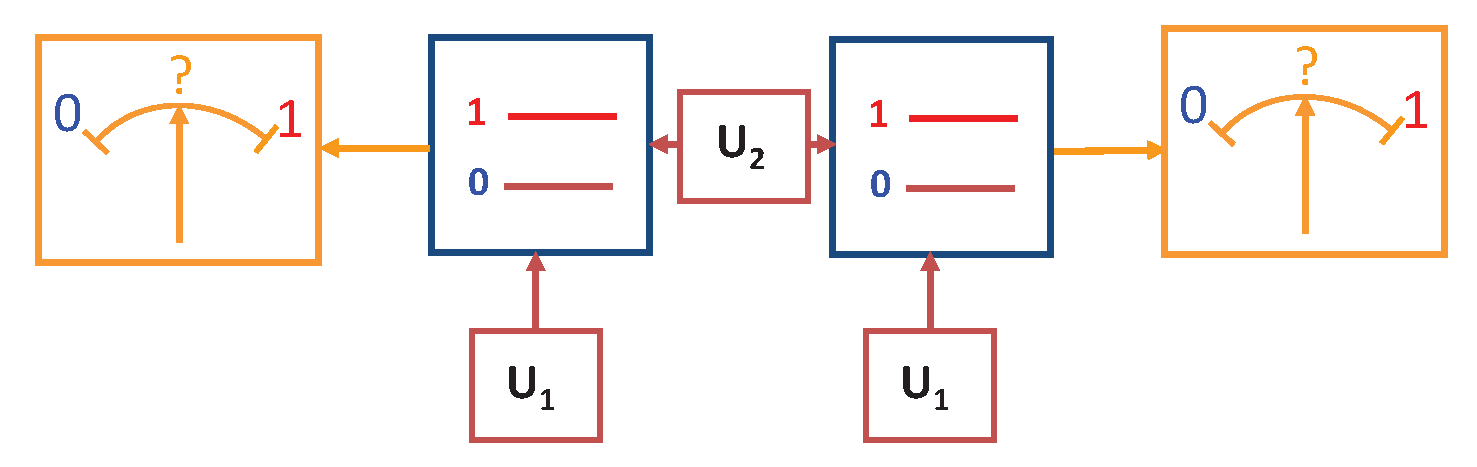
\includegraphics[width=8cm]{Fig1}

\caption{\label{fig:blueprint}Schematic blueprint of a quantum processor based
on quantum gates, represented here in the two-qubit case relevant
for our experiment. A quantum processor consists of a qubit register
that can perform any unitary evolution needed by an algorithm under
the effect of a universal set of quantum gates (single qubit gate
$U_{1}$ , two-qubit gate $U_{2}$). Ideally, all the qubits may be
read projectively, and may be reset.}



\end{figure}


%
\begin{figure}
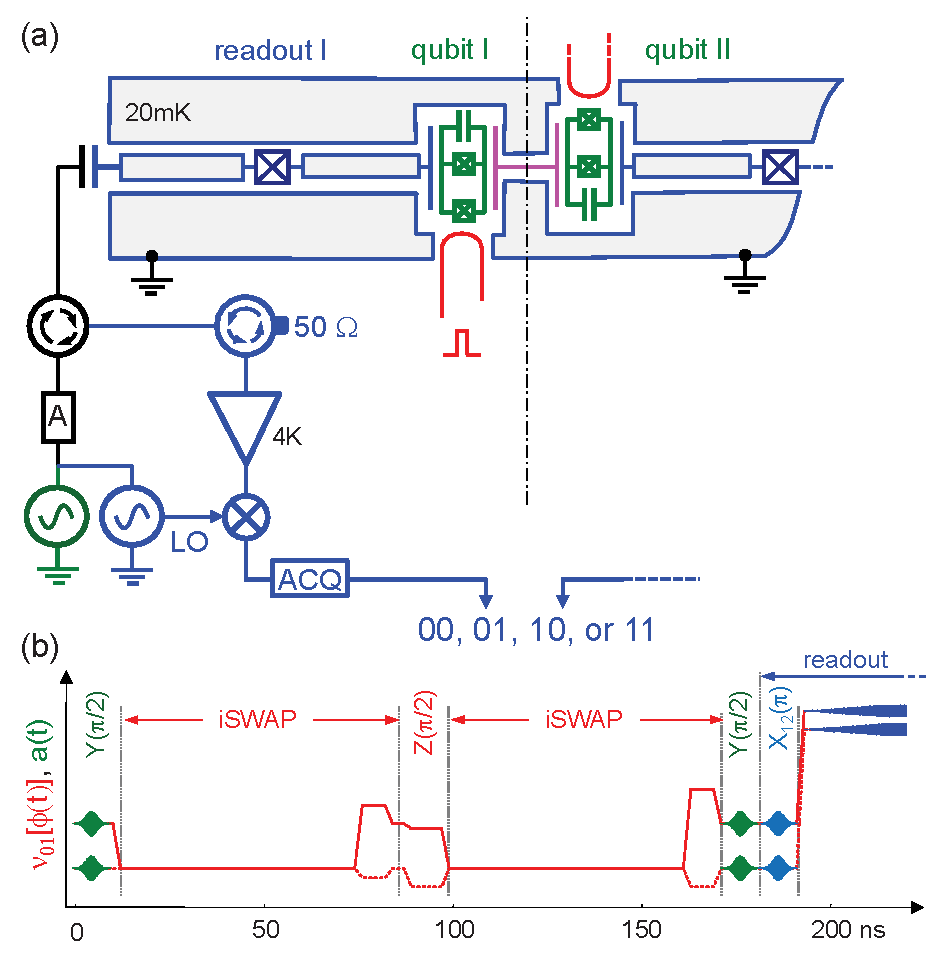
\includegraphics[width=8.5cm]{Fig2} \caption{\label{fig:circuittomo} Electrical scheme of the two qubit circuit
operated and typical sequence during processor operation. (a) two
tunable transmon qubits (green) are capacitively coupled. Their frequency
is controlled by the flux induced in their SQUID loop by a local current
line (in red). The coupling capacitance (in magenta) yields a swapping
evolution between the qubits when on resonance. Each transmon is embedded
in a non-linear resonator used for single-shot readout. Each reflected
readout pulse is routed to a cryogenic amplifier through circulators,
homodyned at room temperature and acquired digitally, which yields
a two-bit outcome. (b) Typical operation of the processor showing
the resonant microwave pulses $a(t)$ applied to the qubits (green)
and to the readouts (blue), on top of the DC pulses (red lines) that
vary the transition frequencies of qubit $I$ (solid) and $II$ (dashed).
With the qubits tuned at a first working point for single qubit gates,
resonant pulses are applied for performing X and Y rotations, and
small flux pulses are applied for Z rotations; qubits are then moved
to the interaction point for two-qubit gate operations. Such sequences
can be combined as needed by the algorithm. Qubits are then moved
to their initial working point for applying tomography pulses and
a $\left|1\right\rangle \rightarrow\left|2\right\rangle $ pulse that
$X_{12}(\pi)$ increases readout fidelity; they are finally moved
at the readout working point and read. }

\end{figure}


The scheme and the operation mode of our processor is shown in Fig.~\ref{fig:circuittomo}.
Two tunable transmon qubits coupled by a fixed capacitor, are embedded
in two identical control and readout sub-circuits. The Hamiltonian
of the two qubits $\left\{ I,II\right\} $ is $H/h=\left(-\nu_{I}\sigma_{z}^{I}-\nu_{II}\sigma_{z}^{II}+2g\sigma_{y}^{I}\sigma_{y}^{II}\right)/2$,
where $\sigma_{x,y,z}$ are the Pauli operators, $\nu_{I,II}$ the
qubit frequency controlled by the flux applied to each transmon SQUID
loop with a fast ($0.5\,\mathrm{GHz}$ bandwidth) local current line,
and $g=4.6\:\mathrm{MHz\ll\nu_{I,II}}$ the coupling frequency controlled
by the coupling capacitance. The achieved frequency control allows
us to place the two transmons on resonance during times precise enough
for performing the universal two-qubit gate \textcolor{black}{$\sqrt{iSWAP}$}
\cite{processor} and the exchange gate\textcolor{black}{{} $iSWAP$}
used in this work. The qubit frequencies are tuned to different values
for single qubit manipulation, two-qubit gate operation, and readout.
The readout is independently and simultaneously performed for each
qubit using the single-shot method of \cite{mallet}. It is based
on the dynamical transition of a non-linear resonator \cite{siddiqi,metcalfe}
that maps the quantum state of each transmon to the bifurcated/non
bifurcated state of its resonator,  which yields a binary outcome
for each qubit. This readout method is potentially non-destructive,
but its non-destructive character is presently limited by relaxation
during the readout pulse. In order to further improve the readout
fidelity, we resort to a shelving method that exploits the second
excited state of the transmon. For this purpose, a microwave pulse
that induces a transition from the state $\left|1\right\rangle $
towards the second excited state $\left|2\right\rangle $ of the transmon
is applied just before the readout pulse as demonstrated in \cite{mallet}.
This variant does not alter the non-destructive aspect of the readout
method since an extra pulse bringing state $\left|2\right\rangle $
back to state $\left|1\right\rangle $ could be applied after readout.
Although the readout contrast achieved with this shelving method and
with optimized microwave pulses reaches $0.88$ and $0.89$ for the
two qubits respectively, the values achieved at working points suitable
for processor operation are lower and equal to $0.84$ and $0.83$.
The readout outcome probabilities for all input states of the two-qubit
register are given in the Supplementary Information S4, with a discussion
of the error sources.

In order to characterize the evolution of the quantum register during
the algorithm, we determine its density matrix by state tomography.
For this purpose, we measure the expectation values of the extended
Pauli set of operators $\left\{ \sigma_{X}I,..,\sigma_{Z}\sigma_{Z}\right\} $
by applying the suitable rotations just before readout and by averaging
typically $10^{4}\:$times. Note that the readout errors, which can
be well-characterized, are corrected when determining the expectation
value of the Pauli set, and thus do not contribute to tomography errors
as explained in \cite{processor}. The density matrix $\rho$ is then
taken as the acceptable positive-semidefinite matrix that, according
to the Hilbert-Schmidt distance, is the closest to the possibly non
physical one derived from the measurement set. In order to characterize
the fidelity of the algorithm at all steps, we use the state fidelity
$F=\left\langle \psi\left|\rho\right|\psi\right\rangle $ with $\left|\psi\right\rangle $
the ideal quantum state at the step considered; $F$ is in this case
the probability for the qubit register to be in state $\left|\psi\right\rangle $. 

The Grover search algorithm \cite{search} consists in retrieving
a particular basis state in a Hilbert space of size $N$ using a function
able to discriminate it from the other ones. This function is used
to build an oracle operator that tags the searched state. Starting
from the superposition $\left|\phi\right\rangle $ of all register
states, a unitary sequence that incorporates the oracle operator is
repeated about $\sqrt{N}$ times, and eventually yields the searched
state with a high probability. The implementation of Grover's algorithm
in a two-qubit Hilbert space often proceeds in a simpler way \cite{grov_Chuang,grov_Fourier_Optics,grov_Jones,grov_optics,grov_Rydberg,grov_trapped_ions}
since the result is obtained with certainty after a single algorithm
step. The algorithm then consists of an encoding sequence depending
on the searched state, followed by a universal decoding sequence that
retrieves it. Grover's algorithm thus provides a simple benchmark
for two-qubit processors. Its implementation with our quantum processor
is shown in \textcolor{black}{Fig.~\ref{fig:operation}(a). First,
the superposed state $\left|\phi\right\rangle $ is obtained by applying
$\pi/2$ rotations around the $Y$ axis for the two qubits. The oracle
operator $O_{uv}$ tagging the two-qubit state $\left|uv\right\rangle \equiv\left|u\right\rangle _{I}\otimes\left|v\right\rangle _{II}$
to be searched is then applied to state $\left|\phi\right\rangle $.
Each $O_{uv}$ consists of a $\mathit{\mathrm{\mathit{iSWAP}}}$ gate
followed by a $Z(\pm\pi/2)$ rotation on each qubit, with the four
possible sign combinations $(-,-)$, $(+,-)$ , $(-,+)$ , and $(+,+)$
corresponding to $uv=00$, $01$, $10$, and $11$, respectively.
In the algorithm we use, as in \cite{dicarlo}}, the encoding is a
phase encoding. When applied to $\left|\phi\right\rangle $, each
oracle operator inverts the sign of the component corresponding to
the state it tags, respectively to the other ones. The density matrix
after applying the oracle ideally takes a simple form: the amplitude
of all coefficients is $1/4$, and the phase of an element $\rho_{rs}$
is $\varphi_{rs}=\pi(\delta_{rt}+\delta_{st})$, where $t$ corresponds
to the state tagged by the oracle operator.  The state tomography
performed after applying the oracle, shown in Fig.~\ref{fig:operation}(b),
is in good agreement with this prediction. More quantitatively, we
find that after having applied the oracle operator, the intermediate
fidelity is $F_{int}=0.87$, $0.80$, $0.84$, and $0.82$, respectively.
We attribute the difference with the ideal density matrix to small
gate errors, to decoherence, and to small errors of the tomography
pulses. The last part of the algorithm consists in transforming the
obtained state in the searched state irrespectively of it, or equivalently
to transform the phase information distributed over the elements of
the density matrix in a weight information with the whole weight on
the searched state. This operation is readily performed by applying
a $\mathrm{\mathit{iSWAP}}$ gate followed by $Y(\pi/2)$ rotations
for both qubits. We find that the fidelity of the density matrix at
the end of the algorithm is $F_{final}=0.70$, $0.62$, $0.67$, and
$0.66$ respectively. This fidelity $F_{final}$ gives the success
probability one would obtain assuming no errors when reading the qubit
register at the end of the algorithm. 

We now consider the success probability obtained after a single run,
which probes the quantum speed-up actually achieved by the processor.
We find (see Fig.~\ref{fig:operation}) that our processor does yield
the correct answer with a success probability $P_{S}=0.67$, $0.55$,
$0.62$, and $0.52$ for the four basis states, which is smaller than
the density matrix fidelity $F_{final}$. One notices that the difference
between $F_{final}$ and $P_{S}$, mostly due to readout errors, slightly
depends on the searched state: the larger the energy of the searched
state, the larger the difference. This dependence is well explained
by the effect of relaxation during the readout pulse, which is the
main error source at readout, the second one being readout crosstalk.
One also notices that the outcome errors are distributed over all
the wrong answers. To summarize, the error in the outcome of Grover's
algorithm originate both from small unitary errors accumulated during
the algorithm, and from decoherence during the whole sequence, in
particular during the final readout. 

%
\begin{figure}[H]
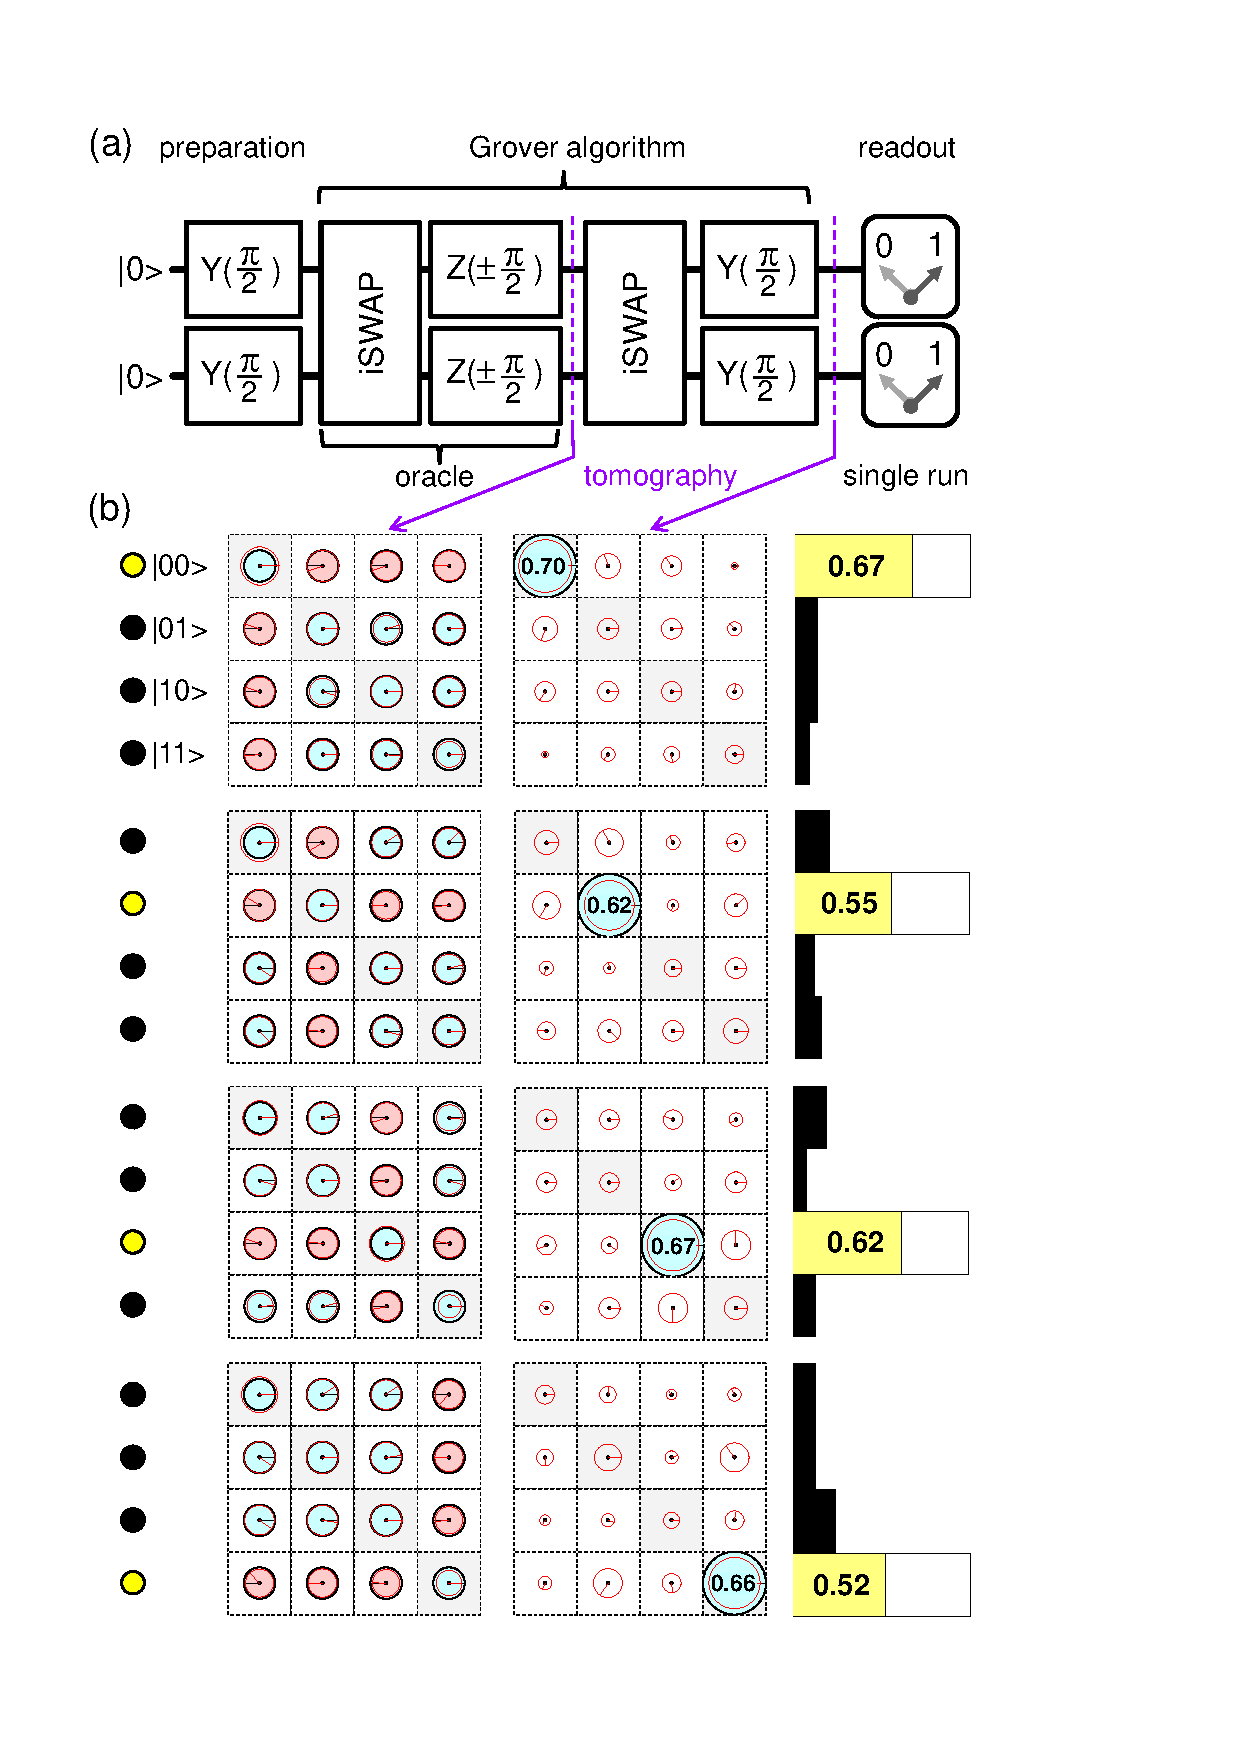
\includegraphics[width=8.5cm]{Fig3} \caption{\label{fig:operation} (a) Experimental sequence used for implementing
the Grover search algorithm on four objects. First, $Y(\pi/2)$ rotations
are applied to produce the superposition $\left|\phi\right\rangle =(1/2){\textstyle \sum_{u,v}\left|uv\right\rangle }$
of all basis states; then one of the four possible oracle (corresponding
to the four sign combinations of the Z rotations) is applied. The
tagged state is then decoded in all cases using a $iSWAP$ operation
followed by $Y(\pi/2)$ rotations. (b) State tomography at two steps
of the algorithm and success probability after a single run. The yellow
dot on the left marks the basis state tagged by each oracle operator
used. After applying the oracle, the information on the tagged state
is encoded in the phase of six particular elements of the density
matrix $\rho$. After decoding, the tagged state should be the only
matrix element present in $\rho$. The amplitude of each matrix element
is represented by a disk (black for the ideal density matrix, red
for the measured one) and its phase by a radius (as well as a filling
color for the ideal matrice). The probability distribution of the
single-run readout outcomes is indicated on the right (yellow box
for the correct answer, filled dark boxes for the wrong ones).}

\end{figure}


\textcolor{black}{We now discuss the significance of the obtained
results in terms of quantum information processing. The achieved success
probability is smaller than the theoretically achievable value $1$,
but nevertheless sizeably larger than the value of $0.25$ obtained
by running once the classical algorithm that consists in making a
random trial. From the point of view of a user that would search which
unknown oracle picked at random has been given to him, the fidelity
of the algorithm outcome is $F_{o}=0.57$, $0.63$, $0.57$, and $0.59$
for the $00$, $01$, $10$, and $11$ outcomes respectively, as explained
in the Supplementary Information S5. Despite the presence of errors,
this result demonstrates the quantum speed-up for Grover's algorithm
when searching in a Hilbert space with small size $N=4$. Demonstrating
the $\sqrt{N}$ speed-up for Grover's algorithm in larger Hilbert
spaces requires a qubit architecture more scalable than the present
one, which presently is a major challenge in the field. }

\textcolor{black}{In conclusion, we have demonstrated the operation
of the Grover search algorithm in a superconducting two-qubit processor
with single-shot non destructive readout. This result indicates that
the quantum speed-up expected from quantum algorithms is within reach
of superconducting quantum bit processors.}
\begin{thebibliography}{22}
\bibitem{search}L.K. Grover, Proceedings, 28th Annual ACM Symposium
on the Theory of \textcolor{black}{Computing}, 1996, p. 212; and Am.
J. Phys., \textbf{69,} 769 (2001).

\bibitem{Shor}P.W. Shor, Proceedings, 35th Annual Symposium on Foundations
of Computer Science, IEEE Press, Los Alamitos, CA, (1994); and SIAM
J. Comp., 26, 1484, (1997).

\bibitem{NielsenChuang}M. A. Nielsen and I. L. Chuang, Quantum Computation
and Quantum Information (Cambridge University Press, Cambridge, UK,
2000).

\bibitem{QC}T.D. Ladd et al., Nature \textbf{\textcolor{black}{464}},
45 (2010).

\bibitem{divincenzo}D.P. DiVincenzo, Fortschritte der Physik \textbf{\textcolor{black}{48}},
771-784 (2000).

\bibitem{Transmon Koch}J. Koch\emph{ et al.}, Phys. Rev. A \textbf{76},
042319 (2007).

\bibitem{TransmonSchreier} J.A. Schreier \emph{et al.}, Phys. Rev.
\textbf{B77}, 180502 (2008).

\bibitem{box}Y. Nakamura, Yu. A. Pashkin, and J. S. Tsai1, Nature
\textbf{398}, 786 (1999).

\bibitem{DeutschJozsa}D. Deutsch and R. Jozsa, Proc. R. Soc. London
1A, \textbf{439}, 553 (1992). 

\bibitem{dicarlo} L. DiCarlo et al., Nature \textbf{467}, 574 (2010).

\bibitem{yamamoto} T. Yamamoto et al., Phys. Rev. \textbf{B 82},
184515 (2010).

\bibitem{mariantoni}M. Mariantoni \emph{et al.}, Science DOI:10.1126,
(2011); arXiv:1109.3743.

\bibitem{processor}A. Dewes et al., submitted to Phys. Rev. Lett;
arXiv:1109.6735.

\bibitem{mallet}F. Mallet\emph{ et al.}, Nature Physics \textbf{5},
791 (2009).

\bibitem{siddiqi}I. Siddiqi \emph{et al.}, Phys. Rev. Lett. \textbf{93},
207002 (2004).

\bibitem{metcalfe}M. Metcalfe\emph{ et al.}, Phys. Rev. B 76, 174516
(2007).

\bibitem{grov_Jones}J.A. Jones, M. Mosca, and R.H. Hansen, Nature
\textbf{393}, 344 (1998).

\bibitem{grov_Chuang} I.L. Chuang, N. Gershenfeld, and M. Kubinec,
Phys. Rev. Lett. \textbf{80}, 3408 (1998).

\bibitem{grov_trapped_ions} K.A. Brickman \emph{et al.}, Phys. Rev.
\textbf{A 72}, 050306, (2005).

\bibitem{grov_Fourier_Optics} N. Bhattacharya \emph{et al.}, Phys.
Rev. Lett. \textbf{88}, 137901 (2002).

\bibitem{grov_optics}P. Walther \emph{et al.}, Nature \textbf{434},
169 (2005).

\bibitem{grov_Rydberg}J. Ahn, T.C. Weinacht, and P.H. Bucksbaum,
Science \textbf{287}, 463 (2000).
\end{thebibliography}

\end{document}
